\subsection{Environmental Transitions} 
Figure \ref{fig:trans} depicts the average transition between environments in different homogenous runs. To compute this typical transition we averaged phenotype disturbance calculated at iterations $[t-40; t + 40] \forall t \in T_r	
\ge 5000$ where $T_r$ is the set of every iteration of the run $r$ such that a transitions between environments occurs, i.e. $E(t) \ne E(t+1)$. Figure  \ref{fig:transonly} shows the different average transitions of ScF genotypes tested a homogeneous test with the same fluctuations. We can see that phenotypes of the genotypes collected later in the evolutionary process are less sensitive to environmental fluctuations. Conversely, as reported of Figure \ref{fig:transli}, the phenotypes of genotypes from SF keep the same high sensitivity regardless of the iteration in which they were collected. Finally the figures \ref{fig:transst} and \ref{fig:transstest} compare the average transitions in homogeneous test with ScF and SF of genotypes collected at iteration 500000 in the four different configurations. Again, it can be seen there that the phenotype of ScF is much more stable than others in its original environment. On the contrary, tested in SF this genotype is very sensitive to transitions. High sensitivity to fluctuations includes both individuals which developed plasticity and those which fail to resist the environement fluctuations.


\begin{figure}[H]
\begin{subfigure}{.25\textwidth}
  \centering
  \includegraphics[width=.7\linewidth, angle =-90]{img/Sucavg499999variationb.eps}
  \caption{SF on genotypes from i:50000.}
  \label{fig:transst}
\end{subfigure}%
\begin{subfigure}{.25\textwidth}
  \centering
  \includegraphics[width=.7\linewidth, angle =-90]{img/SucavgvarValidvariationb.eps}
  \caption{SF on genotypes from SF.}
  \label{fig:transli}
\end{subfigure}

\begin{subfigure}{.25\textwidth}
  \centering
  \includegraphics[width=.7\linewidth, angle =-90]{img/Sucavg499999variationSmallb.eps}
  \caption{ScF on genotypes from i:50000.}
  \label{fig:transstest}
\end{subfigure}%
\begin{subfigure}{.25\textwidth}
  \centering
  \includegraphics[width=.7\linewidth, angle =-90]{img/SucavgvarSmallValidvariationSmallb.eps}
  \caption{ScF on genotypes from ScF.}
  \label{fig:transonly}
\end{subfigure}
\caption{\textbf{phenotype disturbance} : Average transition between environment in different types of homogenous test.}
\label{fig:trans}
\end{figure}


\subsection{Phenotypic Diversity} 



\begin{figure}
\begin{subfigure}{.25\textwidth}
  \centering
  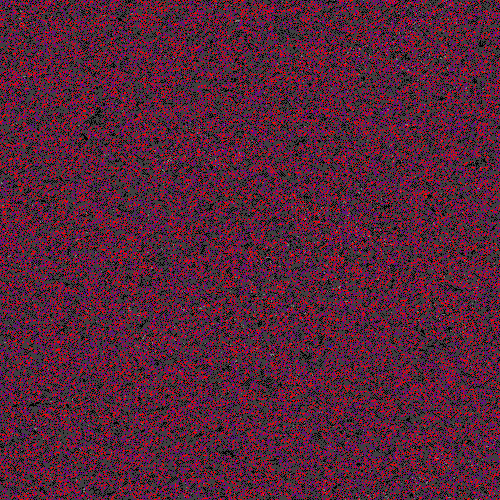
\includegraphics[width=.9\linewidth]{img/stable495000}
  \caption{SE}
\end{subfigure}%
\begin{subfigure}{.25\textwidth}
  \centering
  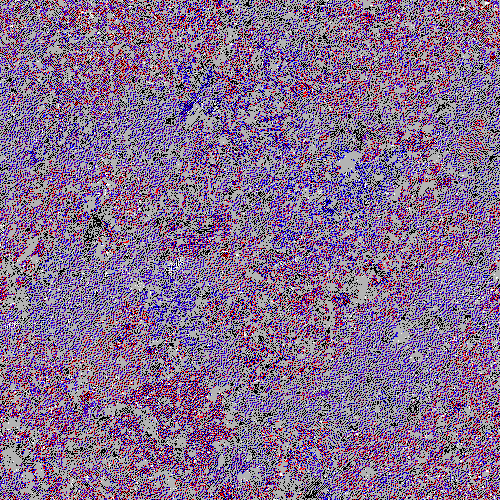
\includegraphics[width=.9\linewidth]{img/var495000}
  \caption{SF}
\end{subfigure}

\begin{subfigure}{.25\textwidth}
  \centering
  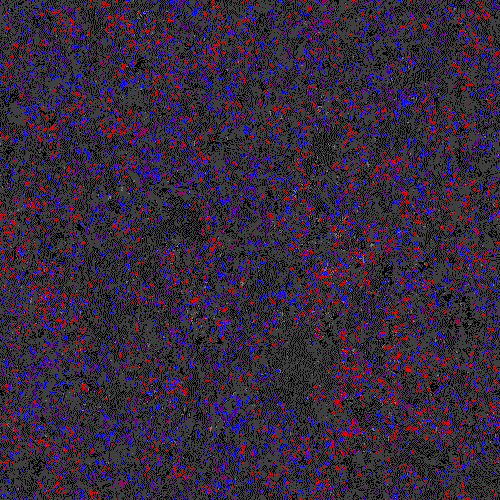
\includegraphics[width=.9\linewidth]{img/light495000}
  \caption{LF}
\end{subfigure}%
\begin{subfigure}{.25\textwidth}
  \centering
  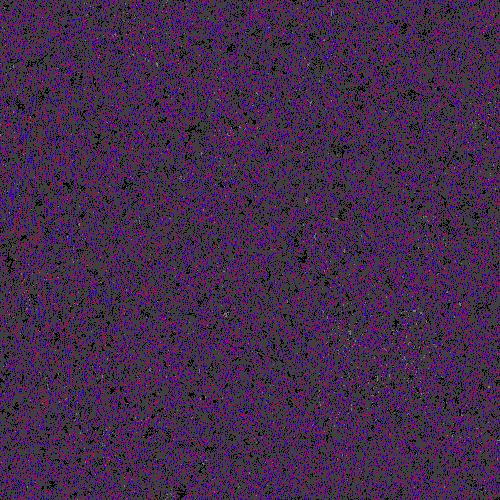
\includegraphics[width=.9\linewidth]{img/small495000}
  \caption{ScF}
\end{subfigure}
\caption{\textbf{Example of CA} gird state repartition (phenotype) at iteration 495000 for the four different configuration. Each cell state is represented by a different color. Black and grey represent respectively cells in \emph{decay} and \emph{quiescent} state.}
\label{fig:phenoexpl}
\end{figure}

The phenotypic diversity measured in Figure \ref{fig:phenodiv} can also be observed relatively easily by simple observation of the cellular automaton as it can be seen with a few examples in Figures \ref{fig:phenoexpl}. 


One distinguishes LF and SF from ScF. These two groups diverge substantially in their characteristic and differ in addition from SE. Individuals from ScF seem to produce stable and robust phenotypes in any environment encountered in ScF. Their adaptations seem essentially be by genotypic mutations and their plasticity seems low. They are also very dependent on their original ecosystem, sometime very distinctive as depicted in Figure \ref{fig:smalldistinctive}, and consequently very little robust in other types of fluctuations, the effect of genotypic mutations is probably enhanced by the reduced size of genotypes. By contrast individuals evolved with LF or SF appear to have a considerable plasticity, their phenotypic diversity is high and it seems likely that phenotypic selection occurs however their genotypic diversity is lower.

\begin{figure}
\begin{subfigure}{.12\textwidth}
  \centering
  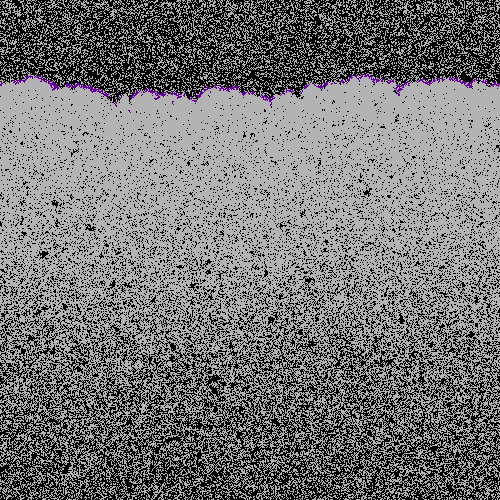
\includegraphics[width=1\linewidth]{img/sm100000}
  \caption{$t=100000$}
\end{subfigure}%
\begin{subfigure}{.12\textwidth}
  \centering
  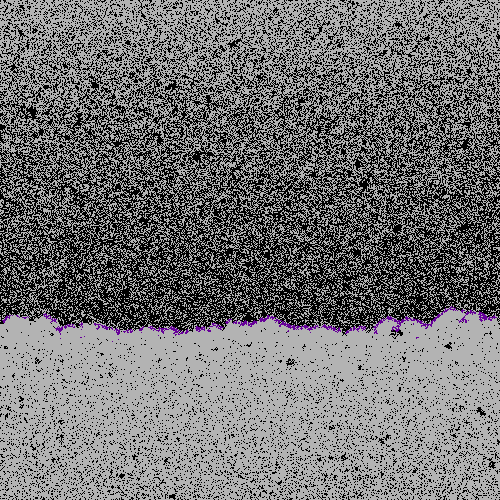
\includegraphics[width=1\linewidth]{img/sm200000}
  \caption{$t=200000$}
\end{subfigure}%
\begin{subfigure}{.12\textwidth}
  \centering
  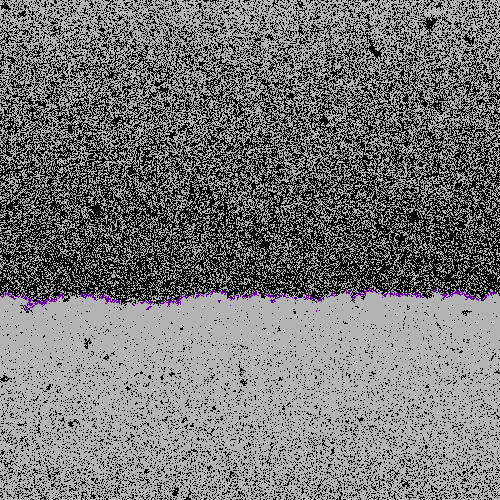
\includegraphics[width=1\linewidth]{img/sm400000}
  \caption{$t=400000$}
\end{subfigure}%
\begin{subfigure}{.12\textwidth}
  \centering
  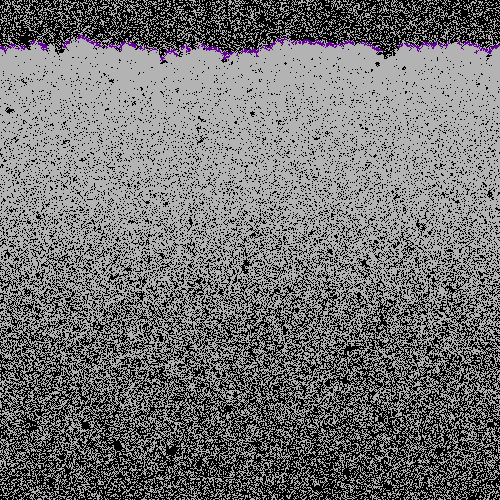
\includegraphics[width=1\linewidth]{img/sm500000}
  \caption{$t=500000$}
\end{subfigure}
\caption{\textbf{Original ScF simulation} having a distinctive waving phenotype, very stable over time $t$, and producing genotypes failing in early iteration of homogeneous test.}
\label{fig:smalldistinctive}
\end{figure}
